\documentclass{beamer}
\usepackage{etex}
\usepackage[latin1]{inputenc}
\usepackage[english]{babel}
\usepackage{helvet,listings}
\usepackage{pgfpages}
\usepackage{graphicx}
\usepackage{wrapfig}
\usepackage{lipsum}
\usepackage{epsfig}
\usepackage{graphicx} % Allows including images
\usepackage{fancybox}
\usepackage{booktabs} % Allows the use of \toprule, \midrule and \bottomrule in tables
\usepackage{caption}
\usepackage{subcaption}
\usepackage{vector}
\usepackage{amsmath}
\usepackage{amssymb}
\DeclareGraphicsExtensions{.pdf,.png,.jpg, .eps}
\usepackage{epstopdf}
\usepackage{braket}
\usepackage{axodraw}
\usepackage[export]{adjustbox}
\usepackage{tikz}
\usepackage{mathtools}
\usepackage{amsmath,bm}
\usepackage{float}
\definecolor{ao(english)}{rgb}{0.0, 0.5, 0.0}
\definecolor{darkpastelpurple}{rgb}{0.59, 0.44, 0.84}
\definecolor{darkpink}{rgb}{0.91, 0.33, 0.5}
\usepackage[font=scriptsize]{caption}
\usepackage{comment}
\usepackage{eso-pic}
\usetheme[compress]{Singapore}
\usepackage{transparent}




\title[Deuteron Electro-Disintegration]{Deuteron Electro-Disintegration At Very High Missing Momenta}
\author{Carlos Yero}
\institute[FIU]{Florida International University \\

\medskip
\textit{cyero002@fiu.edu} % Your email address
}

\date{\today}

% logo of my university
\titlegraphic{
\includegraphics[width=2cm]{fiu_logo.jpg}\hspace*{1.5cm}~%

\includegraphics[width=3.5cm]{jlab_logo.jpg}\hspace*{1.8cm}~%

\includegraphics[width=2cm]{hallc_logo.png}

}


\setbeamertemplate{navigation symbols}{}

\setbeamertemplate{footline}[page number]



\begin{document}

\frame{\titlepage}


\section{Introduction}
\subsection{What is the Deuteron?}

\begin{frame}{What is the Deuteron?}
\begin{itemize}
\begin{footnotesize}
\item Discovered in 1931 by H. Urey
\item Starting point for studying NN interaction
\item Weakly bound state (2.22 MeV/pair)
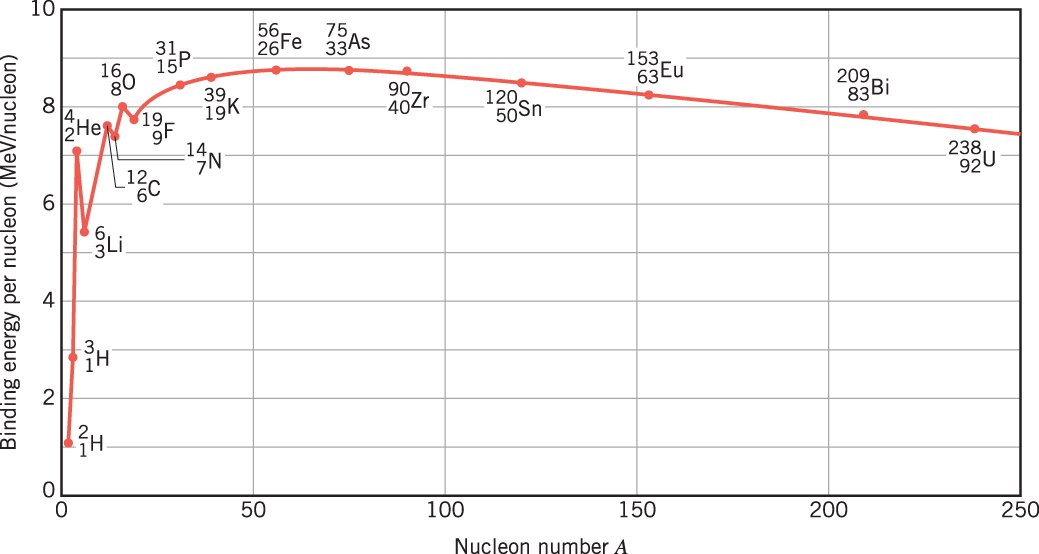
\includegraphics[width=7.5cm]{BE_pernucleon.jpg}
\begin{figure}
\vspace{-3.9cm}\hspace{3.5cm}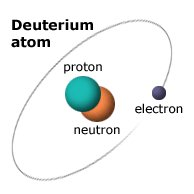
\includegraphics[width=1.9cm]{deuterium.jpg} \hspace{2cm} 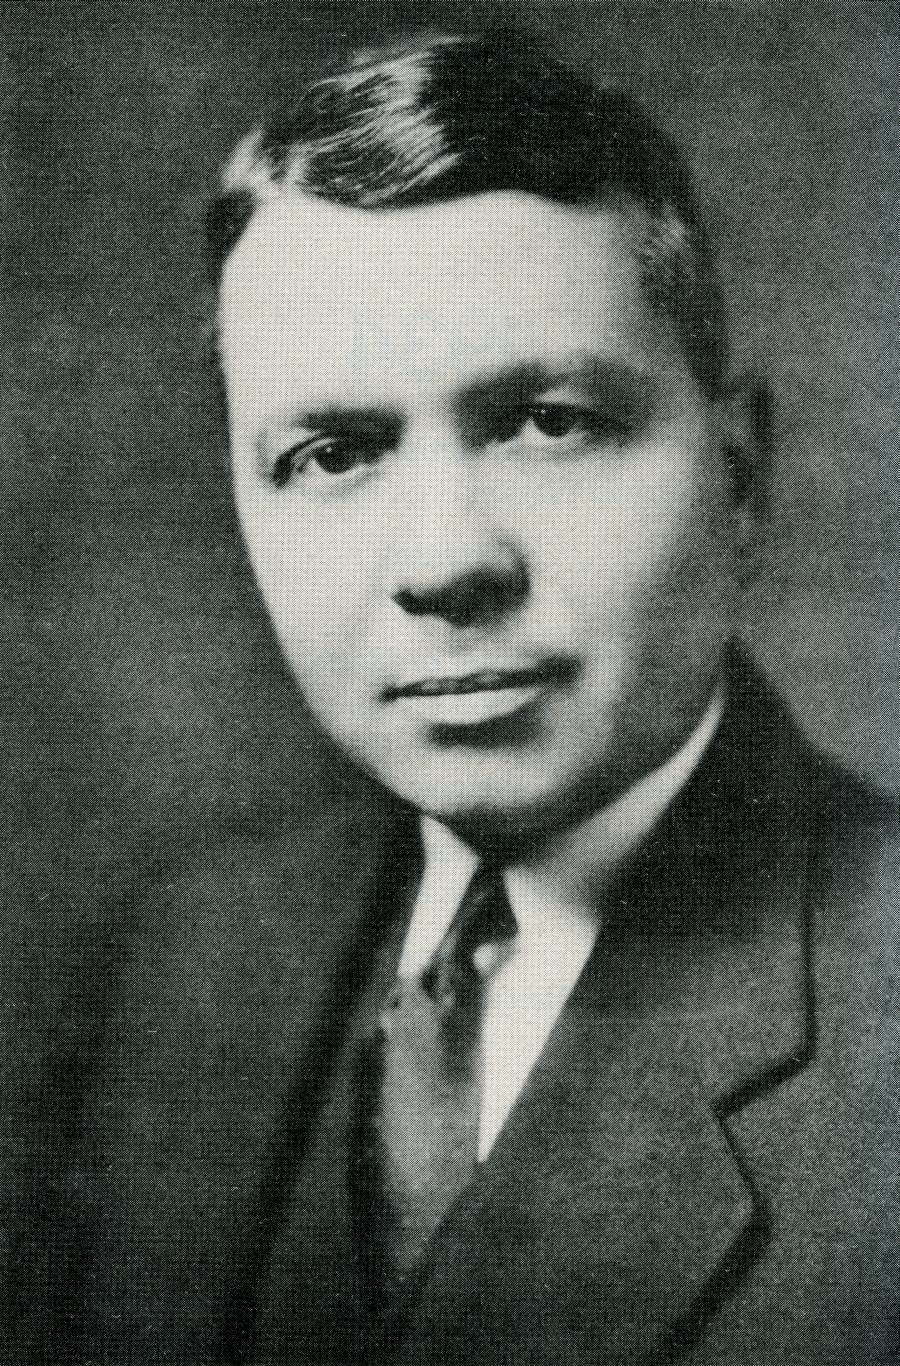
\includegraphics[width=2.2cm]{Harold_Urey.jpg} \\
\end{figure}
\end{footnotesize}
\end{itemize}
\vspace{0.2cm}
\begin{itemize}
\begin{footnotesize}
\item \textcolor{red}{Experiment:} Deuteron has + spatial parity $\implies$ L=0,2,4,$\dots$
\item \textcolor{red}{Experiment:} Total Angular Momentum $J=1\hbar$ $\implies S=s_{p}+s_{n}=\frac{1}{2}\otimes\frac{1}{2}=\textcolor{red}{\boxed{1}}\oplus 0$
\item $\ket{\psi_{D}}=a\ket{^{3}S_{1}(L=0)}+b\ket{^{3}D_{1}(L=2)}$
\item No observed nn or pp bound states (Pauli exclusion, only S=0 singlet state possible for identical fermions)
\item NN interaction is spin dependent 
\end{footnotesize}
\end{itemize}
\end{frame}

\subsection{Deuteron D-State Admixture}

\begin{frame}{Evidence of Deuteron D-state Admixture}
\begin{itemize}
\item Magnetic Dipole Moment \begin{small}$\mu_{d}=\mu^{\text{(orbital)}}_{p}+\mu^{\text{(spin)}}_{p}+\mu^{\text{(spin)}}_{n}$ \end{small} \\ 
\vspace{1mm}
\begin{footnotesize}$\mu^{\textcolor{blue}{tht}}_{d}(^{3}S_{1}(L=0))=\mu_{p}+\mu_{n}=0.879805\mu_{N}$ \hspace{ 1mm } $\mu^{\textcolor{blue}{tht}}_{d}(^{3}D_{1}(L=2))=0.310\mu_{N}$  \\
\vspace{1mm} 
$\mu^{\textcolor{red}{exp}}_{d}=0.85741 \pm 0.00002\mu_{N}$ \end{footnotesize}  
\vspace{3mm}
\item Electric Quadrupole Moment
\begin{itemize}
\item I.I. Rabi measured electric quadrupole moment in D (1939) \\
\item Multipole Expansion: \begin{footnotesize} $\phi(\mathbf{r}) = \phi_{m}(\mathbf{r}) + \phi_{d}(\mathbf{r}) + \phi_{q}(\mathbf{r}) + \cdots$ \\
$\phi(\mathbf{r}) = \sum\limits_{L}\sum\limits_{M=-L}^{L}C_{L}^{M}Y_{L}^{M}(\theta,\phi) = C_{0}^{0}Y_{0}^{0} + C_{2}^{M}Y_{2}^{M}(\theta,\phi)$ \end{footnotesize}  
\end{itemize}
\begin{footnotesize}
\begin{figure}[h!]
\vspace{-0.3cm}\hspace{0.0cm}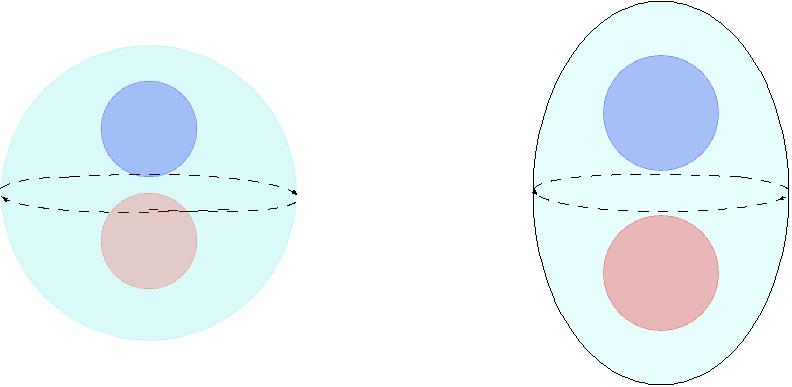
\includegraphics[width=3.0cm]{multipole.jpg} \hspace{2.4cm} 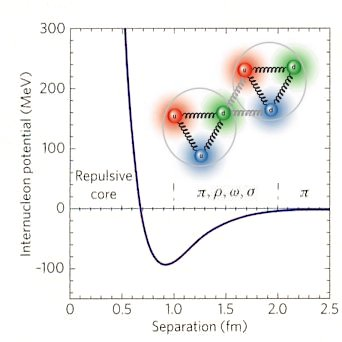
\includegraphics[width=3.1cm]{NN_potential.jpg}
\end{figure}
\hspace{0.7cm}$L=0$ \hspace{1.6cm} $L=2$ \\
\hspace{-0.2cm}$V_{int}=$\hspace{0.1cm}$V_{central}$ \hspace{0.4cm} + \hspace{0.6cm} $V_{non-central}$ $\implies$ tensor force 
\end{footnotesize}
\end{itemize}
\end{frame}

\section{Motivation}

\begin{frame}{Motivation}
\begin{itemize}
\begin{footnotesize}
\item Study Deuteron at short ranges ($\lesssim$ 1fm). \\
\vspace{0.2cm}
High momentum transfers ($Q^{2}$)$\implies$ probe the Deuteron at smaller distances. 
Smaller internucleon distances enables one to access the high momentum components of nucleons \\
\vspace{0.5cm}
\item Extract momentum distributions(not an observable) from cross sections
\vspace{0.5cm}
\item Study transition from hadronic to quark-gluon degrees of freedom \\
\end{footnotesize}
\end{itemize}
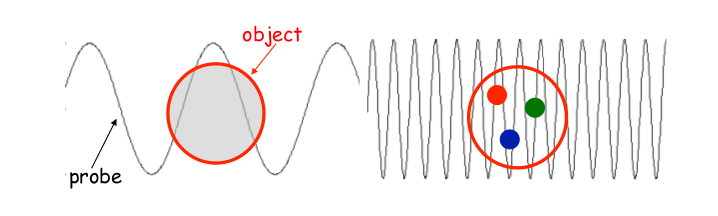
\includegraphics[width=8.0cm]{probe.png}
\end{frame}


\section{Theoretical Framework}

\begin{frame}{Theoretical Framework of D(e,e'p)n}
\begin{columns}
\column{.55\linewidth}
\begin{itemize}
\begin{footnotesize}
\item E.M. Interaction ($\alpha \sim \frac{1}{137}$) 
\vspace{0.5cm}
\item One Photon-Exchange Approximation is valid 
\vspace{0.5cm}
\item virtual photon interacts with Deuteron through a variety of processes
\vspace{0.5cm}
\item preferably, proton absorbs photon and is ejected while neutron recoils without
further interaction (missing neutron momenta is same
as internal momenta) \\
\end{footnotesize}
\end{itemize}
\column{.65\linewidth}
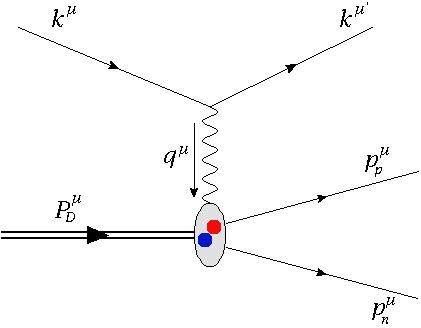
\includegraphics[width=5.0cm]{feynmann.jpg} \\
\begin{footnotesize}
$\mathit{k^{\mu} = (E, \mathbf{k}) \hspace{0.5cm} k^{\mu'}=(E',\mathbf{k'})}$ \\
\vspace{0.1cm}
$\mathit{q^{\mu}=(\omega, \mathbf{q})} $ \\
\vspace{0.1cm}
$\mathit{\omega=E'-E}$,  $\mathit{\mathbf{q}=\mathbf{k'}-\mathbf{k}}$ \\
\vspace{0.1cm}
$\mathit{P^{\mu}_{D}=(M_{D},\mathbf{P_{D}})}$ \\
\vspace{0.1cm}
$\mathit{\mathbf{P_{D}=p_{i,p}+p_{i,n}}=}0$ \\
\vspace{0.1cm}
$\mathit{Q^{2}\equiv-q_{\mu}q^{\mu}=4EE'\sin^{2}\Big(\frac{\theta_{e}}{2}\Big)}$
\end{footnotesize}
\end{columns}
\end{frame}

\subsection{Plane Wave Impulse Approximation}

\begin{frame}{Plane Wave Impulse Approximation (PWIA)}
\begin{columns}
\column{.55\linewidth}
\begin{itemize}
\begin{footnotesize}
\item virtual photon is completely absorbed by one of the nucleons
\vspace{0.5cm}
\item the other nucleon is a spectator
\vspace{0.5cm}
\item final state particles treated as plane waves (free particles)
\vspace{0.5cm}
\item \textcolor{darkpastelpurple}{process in which neutron absorbs photon (+PWBA) is suppressed only for
proton momenta significantly higher than missing momenta.}
\end{footnotesize}
\end{itemize}
\column{.85\linewidth}
\includegraphics[width=5.0cm]{PWIA.eps} \\
\vspace{1.0cm}
\textcolor{darkpastelpurple}{\boxed{\includegraphics[width=5.0cm]{PWBA.eps}}} \\
\end{columns}
\end{frame}

\subsection{Final State Interactions (FS1)}

\begin{frame}{Final State Interactions (FSI)}
\begin{columns}
\column{.55\linewidth}
\begin{itemize}
\begin{footnotesize}
\item in final state, the nucleons are at short enough distances ($\sim$ 2 fm)
and continue to interact 
\vspace{0.5cm}
\item eikonal approximation: infinite NN interactions are 
represented by an effective NN interaction amplitude
obtained from NN scattering experiments
\vspace{0.5cm}
\item nucleons re-scatter after interacting
\end{footnotesize}
\end{itemize}
\column{.85\linewidth}
\includegraphics[width=6.8cm]{FSI.eps} \\
\end{columns}
\end{frame}

\subsection{Meson Exchange Currents (MEC)}

\begin{frame}{Meson Exchange Currents (MEC)}
\begin{columns}
\column{.55\linewidth}
\begin{itemize}
\begin{footnotesize}
\item virtual photon couples with exchange meson between nucleons 
\vspace{0.5cm}
\item virtual meson may become real after photon absorption
\vspace{0.5cm}
\item meson exchange propagator is proportional
to $(1+\frac{Q^{2}}{m^{2}_{meson}})^{-1}$ \\
$\implies$ \textcolor{red}{MEC suppressed for $Q^{2}\gg m^{2}_{meson}$}
\end{footnotesize}
\end{itemize}
\column{.85\linewidth}
\includegraphics[width=5.0cm]{MEC.eps} \\
\end{columns}
\end{frame}

\subsection{Isobar Configuration Currents (IC)}

\begin{frame}{Isobar Configuration Currents (IC)}
\begin{columns}
\column{.50\linewidth}
\begin{itemize}
\begin{footnotesize}
\item virtual photon excites nucleon into resonance
\vspace{0.5cm}  
\item resonance de-excites through meson exchange with spectator nucleon
\vspace{0.5cm}
\item for high $Q^{2}$, and $x_{B_{j}}>1$
($x_{Bj}\equiv \frac{Q^{2}}{2M_{p}\omega}$) one is able to
probe the lower $\omega$ region of the quasi-elastic peak
to \textcolor{red}{suppress $\Delta$ or $N^{*}$  resonance production}

\end{footnotesize}
\end{itemize}
\column{.85\linewidth}
\includegraphics[width=5.0cm]{IC.eps} \\
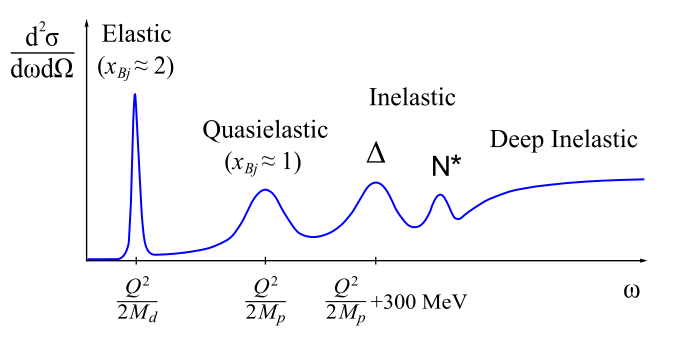
\includegraphics[width=7.0cm]{crosssection_v_energy.png} \\
\end{columns}
\end{frame}

\section{D(e,e'p)n Data}
\subsection{Data from Mainz Microtron (MAMI)}

\begin{frame}
\begin{columns}
\column{.53\linewidth}
\tikz\draw[black,fill=black] (0,0) circle (.5ex); Data \\
\tikz{\draw[red,solid,line width=0.9pt](0,0) -- (10mm,0);} \small Arenh\"{o}vel (FSI+MEC+IC)\\
\tikz{\draw[red,dashed,line width=0.9pt](0,0) -- (10mm,0);} PWIA+FSI+MEC+IC+R  \\
\tikz{\draw[magenta,dotted,line width=0.9pt](0,0) -- (10mm,0);} PWIA+FSI+MEC  \\
\tikz{\draw[blue,dashed,line width=0.9pt](0,0) -- (10mm,0);} PWIA + PWBA  \\
\tikz{\draw[ao(english),dashdotted,line width=0.9pt](0,0) -- (10mm,0);} PWIA+FSI \\
\tikz{\draw[ao(english),dashed,line width=0.9pt](0,0) -- (10mm,0);} PWIA  \\
\vspace{5mm}
MAMI $Q^{2}=0.33$ (GeV/c)$^{2}$\\
Blomqvist et al. PLB 424 (1998) 33
\column{.50\linewidth}
\begin{figure}[t!]
\vspace{-0.5cm}
\hspace{-11.08mm}
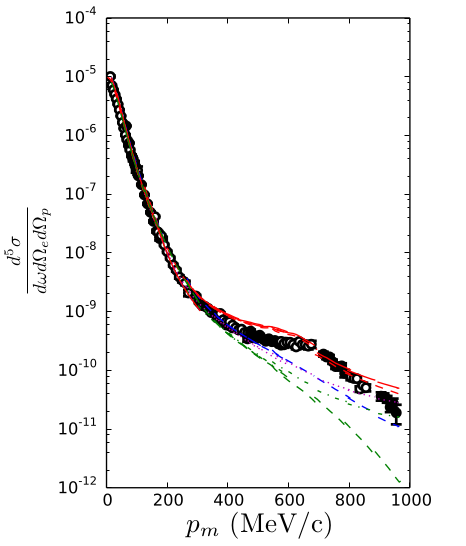
\includegraphics[width=6.0cm]{MAMI.png} 
\end{figure}
\end{columns}
\end{frame}

\subsection{Data from Jefferson Lab (Hall A)}

\begin{frame}
\begin{columns}
\column{.53\linewidth}
\tikz\draw[black,fill=white] (0,0) circle (.5ex); Data (JLAB HallA) \\
\tikz{\draw[black,dashdotted,line width=1.3pt](0,0) -- (10mm,0);} JML (FSI+MEC+IC)  \\
\tikz{\draw[ao(english),dashed,line width=1.3pt](0,0) -- (10mm,0);} JML (FSI)  \\
\tikz{\draw[darkpastelpurple,solid,line width=1.3pt](0,0) -- (10mm,0);} MS using CD-Bonn potential\\
\tikz{\draw[darkpink,dashed,line width=1.3pt](0,0) -- (10mm,0);} JVO\\
\vspace{3mm}
$Q^{2}=3.5$ (GeV/c)$^{2}$ \\
\vspace{1mm}
(a)p$_{m}$=0.2 GeV/c \\
(b)p$_{m}$=0.4 GeV/c \\
(c)p$_{m}$=0.5 GeV/c \\
\vspace{5mm}
W.U. Boeglin et. al \\
PRL 107(2011) 262501
\column{.50\linewidth}
\begin{figure}[t!]
\vspace{-0.5cm}
\hspace{-11.08mm}
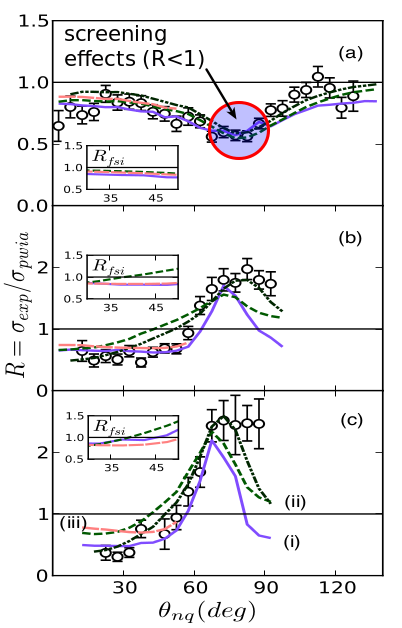
\includegraphics[width=5.5cm]{angular_dist.png} 
\end{figure}
\end{columns}
\end{frame}

\section{12 GeV Upgrade and D(e,e'p)n}
\subsection{High Momentum Spectrometer (HMS) and Super High Momentum Spectrometer (SHMS)}

\begin{frame}{{Hall C 12 GeV Upgrade and D(e,e'p)n}}
\centering
\hspace{1.0cm}\includegraphics[width=10.0cm]{HMS.pdf} 
\end{frame}

\subsection{Simulation of D(e,e'p)n at Hall C}

\begin{frame}
\begin{columns}
\column{.32\linewidth}
\footnotesize
\underline{D(e,e'p)n Kinematics}
$E_{e}=11$ GeV \\
$Q^{2}=4.25$ (GeV/c)$^{2}$ \\
$x_{B_{j}}=1.35$
$p_{m} = 0.5 - 1.0$ GeV/c \\
$\theta_{nq} = 35^{\circ} - 40^{\circ}$ \\
\vspace{5mm}
W.U. Boeglin et. al \\
Int.J.Mod.Phys. E24 \\
(2015) no.03, 1530003 
\column{.68\linewidth}
\begin{figure}[t!]
\hspace{-0.89cm}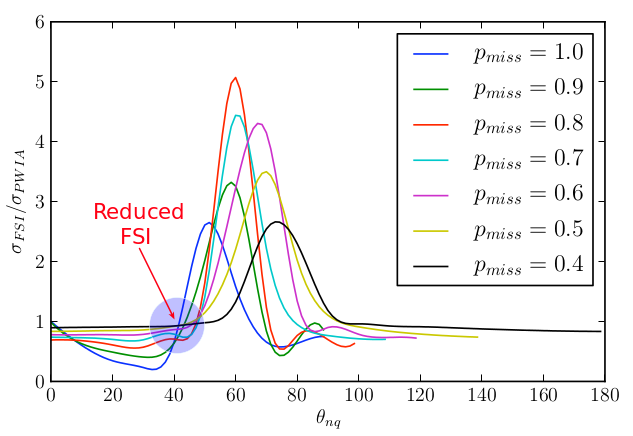
\includegraphics[width=8.18cm]{ang_dist2.png} 
\end{figure}
\end{columns} 
\end{frame}

\section{Conclusion and Future Outlook}

\begin{frame}{Conclusion and Future Outlook}
\begin{footnotesize}
\begin{itemize}
\item $np$ bound state serves as starting point to study the strong nuclear force
\vspace{0.5cm}
\item Investigate NN interaction at sub-fermi distances by using high energy $e^{-}$ probe
\vspace{0.5cm}
\item Previous experiments have shown that final state processes may be minimized in certain kinematic regions
\vspace{0.5cm}
\item There are theoretical expectations that at high $Q^{2}$ and $x_{Bj}>1$, soft two-body processes such as MEC and IC may be suppressed
\vspace{0.5cm}
\item With the 12 GeV Upgrade at HallC, the D(e,e'p)n experiment seeks to explore new kinematic regions (backed by experimental and theoretical support)  
that will enhance PWIA over other processes 
\end{itemize}
\end{footnotesize}
\end{frame}

\section{Acknowledgments}

\begin{frame}{Acknowledgments}
I would like to thank Drs. W. U. Boeglin and M.M. Sargsian for their experimental and theoretical contributions to the study of the Deuteron on this
presentation. \\
\vspace{2cm}
\begin{Huge}
\centerline{Thank You!}
\end{Huge}
\end{frame}

\end{document}
